\chapter{Related Work}

\section{Standard methods for shape detection}

\subsection{Simple Linear Iterative Clustering (SLIC)}

\section{The development of Convolutional neural networks}
Since McCulloch and Pitts created what is acknowledged as the first neural network in 1943, using simple electrical circuits \citep{Mcculloch1990}, they have played an important role in the field of pattern recognition. 

Since the late 1990's the idea of using convolutional operations in these networks has been considered more and more prominent \citep{LeC}, and this approach is still one of the leading research fields within ANN research \citep{Wu2017}. This section will discuss the development of the convolutional neural networks the last two decades.

\subsection{Early adaption of convolutional neural networks}
The earliest attempts of using convolutional operations for pattern and object recognition in neural networks was first done nearly twenty years ago. 

MORE HERE (LeNet)

\subsection{Deep Convolutional Neural Networks}
It was however, not until Alex Krizhevsky, Geoffrey Hinton, and Ilya Sutskever won the ImageNet \footnote{ImageNet is a very large dataset consisting of 15 million labeled, high-resolution images divided into over 22.000 categories.} 2012 competition, that CNNs became acknowledged as one of the most sophisticated approaches for image recognition. Their deep convolutional neural network (commonly called AlexNet) consisted of five convolutional layers, each followed by a pooling layer (max-pooling), and three fully-connected softmax layers \citep{Krizhevsky2012}.  In order to reduce overfitting, the network applied two different methods; Data Augmentation and Dropout layers.

Even though the AlexNet was a big break through for the convolutional neural networks, it was criticized for not presenting a good ground for understanding of what was happening inside the network, thus making it hard to improve. One of the solutions to this problem are the ZF Net, which applies deconvolutional neural networks \citep{Zeiler2011} in order to map the dense feature space produced by a CNN back to its original pixel space \citep{Zeiler2014}. \autoref{fig:deconv} shown how a deconvolutional network can help visualizing the feature space of a CNN.

\begin{figure}[!h]
	\centering
	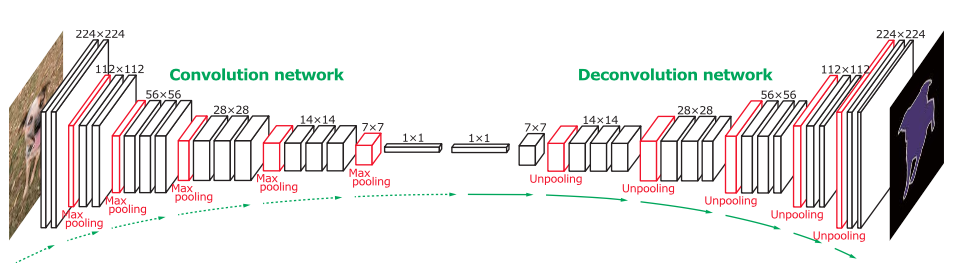
\includegraphics[scale=0.5]{fig/deconv.png}
	\caption{Process of visualizing the feature space of a CNN \citep{Noh2015}}
	\label{fig:deconv}
\end{figure}



\subsection{ZF Net}
\subsection{GoogLeNet}
\subsection{VGGNet}
\subsection{ResNet}

\section{Height estimation form a nadir perspective}

